% =============================================================
% Bilgisayar Mimarisi - Kapak Sayfası
% Konsept: Açılmış işlemci katmanları (transistörden çekirdeğe)
% Görsel: gorseller/kapak-arkaplan-katmanlar.png (Codex imagegen, Eylül 2026)
%   Ham görsel ...-ham.png; alt degrade kapak-degrade.py ile işlenir.
% Eski görsel: gorseller/kapak-arkaplan.png (yerinde duruyor)
% =============================================================

% --- Kapak Renkleri ---
\definecolor{pcbzemin}{RGB}{10, 25, 50}
\definecolor{pcbaltin}{RGB}{205, 175, 100}
\definecolor{pcbacik}{RGB}{230, 210, 150}
\definecolor{pcbbeyaz}{RGB}{245, 245, 240}
\definecolor{kapakamber}{RGB}{242, 184, 76}

% --- Kapak yazı tipi: IBM Plex Sans (yalnız kapakta; iç sayfalar Libertinus) ---
\newfontfamily\kapakyazi{IBMPlexSans-Regular.otf}[BoldFont=IBMPlexSans-SemiBold.otf]


\begin{titlepage}
\thispagestyle{empty}
\null\vfill
\begin{tikzpicture}[remember picture, overlay]

    % === TAM SAYFA ARKA PLAN GÖRSELİ ===
    \begin{scope}
        \clip (current page.south west) rectangle (current page.north east);
        \node[inner sep=0pt] at (current page.center) {%
            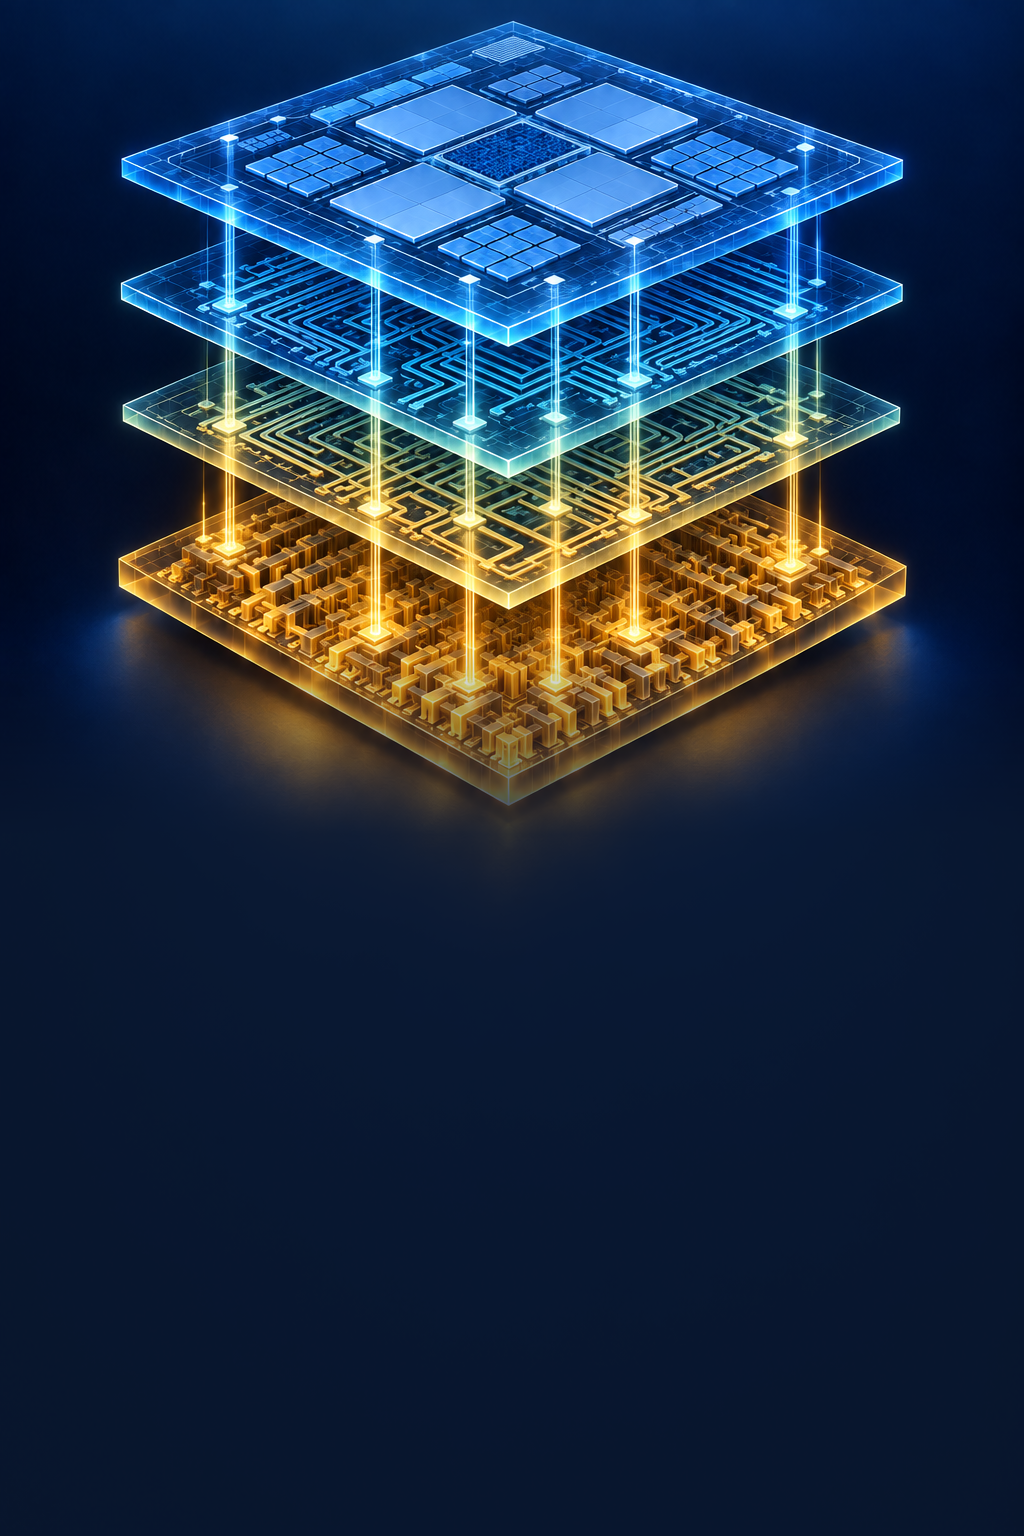
\includegraphics[width=\paperwidth]{gorseller/kapak-arkaplan-katmanlar.png}%
        };
    \end{scope}

    % === ALT BÖLGE: Koyu degrade ===
    % Degrade görselin içine işlenmiştir (kapak-degrade.py). LaTeX'te üst üste
    % saydam şekillerle çizilince yığının amber yansımasında ek yeri çizgileri çıkıyordu.

    % === ÜST VE ALT ŞERİT (ince altın çizgi) ===
    \fill[pcbaltin] (current page.north west) rectangle ([yshift=-1.2mm]current page.north east);
    \fill[pcbaltin] ([yshift=1.2mm]current page.south west) rectangle (current page.south east);

    % === ANA BAŞLIK (IBM Plex Sans, sayfa genişliğinin yarısı) ===
    \node[font=\kapakyazi\fontsize{70}{78}\selectfont\bfseries, text=pcbbeyaz]
        at ([yshift=10.7cm]current page.south) {Bilgisayar};
    \node[font=\kapakyazi\fontsize{70}{78}\selectfont\bfseries, text=pcbbeyaz]
        at ([yshift=8.1cm]current page.south) {Mimarisi};

    % === AMBER AYIRICI ÇİZGİ ===
    \draw[kapakamber, line width=2pt]
        ([yshift=6.75cm, xshift=-5cm]current page.south) -- ++(10cm,0);

    % === ALT BAŞLIK (RISC-V vurgulu) ===
    \node[font=\kapakyazi\fontsize{26}{30}\selectfont, text=pcbbeyaz]
        at ([yshift=5.6cm]current page.south)
        {\textcolor{kapakamber}{\bfseries RISC-V} Tabanlı Yaklaşım};

    % === YAZAR ADI ===
    \node[font=\kapakyazi\fontsize{19}{22}\selectfont, text=pcbbeyaz]
        at ([yshift=3.5cm]current page.south) {Prof.\ Dr.\ Oğuz Ergin};

    % === BASKI BİLGİSİ ===
    \node[font=\kapakyazi\fontsize{13}{16}\selectfont, text=pcbacik]
        at ([yshift=1.7cm]current page.south) {Sürüm \kitapsurum\ \ ·\ \ \the\year};

\end{tikzpicture}
\vfill
\end{titlepage}
